

\documentclass{article}
\usepackage[utf8]{inputenc}
\usepackage{authblk}
\usepackage{setspace}
\usepackage{natbib}
\usepackage{hyperref}
%\usepackage{cite}
\usepackage[margin=1in]{geometry}
\usepackage{array}
\usepackage{graphicx}
\usepackage{caption}
\graphicspath{ {./figures/} }
\usepackage{subcaption}
\usepackage{amsmath}
\usepackage{lineno}
\usepackage{soul}
\usepackage{xcolor}
\sethlcolor{yellow}
\linenumbers

%%%%%%%%%%%%%%%%%
\title{Thesis outline}
\date{\today}
\author{Christophe Rouleau-Desrochers}
\begin{document}
%%%%%%%%%%%%%%%%%%%%%%%%%%%%%%

\maketitle


%<><><><><><><><><><><><><><><><><><><><>
% Introduction
%<><><><><><><><><><><><><><><><><><><><>
\section{Introduction}

% ============================
% 1. CC  X Phenology
% ============================
\subsection{Climate change impacts on tree phenology} 
Climate change impacts on biological systems and how phenological trends are already shifting with warming temperatures. 
\begin{enumerate}
% 1)
	\item  Trends of spring and autumn phenological events and their drivers \citep{walther_ecological_2002}
% 2)
	\item Evidence of declining sensitivity to warming, predominance of winter temperature in spring phenological responses (\textit{to work on}) \citep{ettinger_winter_2020}
%Long-term trends suggest that the pace of spring events advancement is slowing down.  Counterinteraction of warmer winters that delays spring phenology because of non-met chilling requirements, which increase forcing requirements --> later budburst 
%Include in main text: Deacclimatation forms during spring
%Autumn phenological events are delayed, but the trend is not as clear as spring's. Description of mechanistic drivers of autumn phenology vs spring
% Include in main text: We have a good mechanistic understanding of the drivers that lead plants to leaf out early, but we don't for Autumn. \textit{Maybe talk about why the trend isn't clear (e.g. monitoring leaf fall and colouring is hard. Can be highly influenced by a single episode of wind, precipitation or frost (Gunderson, 2012)}  
% See note: Correcting for non-linearity removes evidence of declining sensitivities with warming
% Interaction of chilling, forcing and photoperiod: Ettinger 2020.
% See:Photoperiod perception interaction with warming requirements (Zohner 2016)
% 3)
	\item Mechanisms that could limit growth despite having a longer growing season: \\
	\par
		\textbf{3.1. Spring frosts} \\
\resizebox{\textwidth}{!}{
\begin{tabular}{|>{\raggedright\arraybackslash}p{4cm}|p{12cm}|}
\hline
\textbf{} & \multicolumn{1}{c|}{\textbf{}} \\
\hline

\textbf{Mechanisms} & Early warm spells $\rightarrow$ early leaf out $\rightarrow$ hard frost ($<$-2Celsius) $\rightarrow$ tissue death = loss of photosynthetic capacity \cite{polgar_leafout_2011}; Response: second cohort of leaves are more efficient and mitigate carbon sequestration loss \cite{reinmann_compensatory_2023} \\
\hline
\textbf{Global trend of occurrence} & Most vulnerable regions are the ones with no past risk of occurrence (); $\uparrow$ in Europe and East Asia, but $\downarrow$ North America; Global trend is controversial \cite{reinmann_compensatory_2023} \\
\hline
\textbf{Consequences (Individual and Ecosystem level consequences)} & Loss of vegetative tissue = $\downarrow$ photosynthesis = $\downarrow$ and remobilization of NSC to repair damaged tissues = $\downarrow$ secondary growth (Meyer24); Loss of reproductive tissue (higher flower mortality) (REF); Costs for orchards and stuff \cite{reinmann_compensatory_2023} \\
\hline
\textbf{Differences across species/provenance} & \\
\hline
\end{tabular}
} 

\clearpage
	\textbf{3.2. Drought} \\
\resizebox{\textwidth}{!}{
\begin{tabular}{|>{\raggedright\arraybackslash}p{4cm}|p{12cm}|}
\hline
\textbf{} & \multicolumn{1}{c|}{\textbf{}} \\
\hline
\textbf{Mechanisms} & — Hot temperature + low precipitation (aka global-change-type drought \cite{tyree_xylem_2002})= $\uparrow$ evapotranspiration$\rightarrow$ less water in soil $\rightarrow$ cavitation $\rightarrow$ embolism $\rightarrow$ hydraulic failure \cite{tyree_xylem_2002} = tissue death \citep{choat_triggers_2018}; 

— Earlier spring phenology = longer GS $\rightarrow$ increases vegetative growth $\rightarrow$ increases evapotranspiration $\rightarrow$ increases drawdown of soil moisture = progressive water stress \cite{li_widespread_2023}

— Long-term vs short-term stomatal responses and consequences on tissue death \citep{choat_triggers_2018}; 

— Recovery and its determinants \citep{choat_triggers_2018,li_widespread_2023}\\
\hline
\textbf{Global trend of occurrence} & — $\uparrow$ precipitation anomalies since 1990 \cite{trenberth_global_2014};  

— Models often exclude PDO/ENSO which limit the capacity to attribute increasing droughts to CC  \cite{trenberth_global_2014}; 

— Weak evidence of detection and attribution of changes in meteorological drought since the mid-20th century \cite{intergovernmental_panel_on_climate_change_detection_2014}; 

— Using a spacial, model-based perspective, anthropogenic forcing increased the frequency, duration and intensity of SPI-based droughts for Americas, Mediterreanean, W/S Africa and E Asia \cite{chiang_evidence_2021} \\
\hline
\textbf{Consequences (Individual and Ecosystem level consequences)} & — Recurring droughts may limit trees' ability to recover from other types of stress.

—Tree mortality (E.g. Texas and California extreme droughts are estimated to have killed 300 and 102 million trees \cite{li_widespread_2023}\\
\hline
\textbf{Differences across species/provenance} &  \\
\hline
\end{tabular}
} \\
\par

\textbf{3.3. Heat waves : \textit{needs to be filled}}\\
\resizebox{\textwidth}{!}{
\begin{tabular}{|>{\raggedright\arraybackslash}p{4cm}|p{12cm}|}
\hline
\textbf{} & \multicolumn{1}{c|}{\textbf{}} \\
\hline
\textbf{Mechanisms} &  \\
\hline
\textbf{Trend mechanism} &  \\
\hline
\textbf{Global trend of occurrence} &  \\
\hline
\textbf{Consequences (Individual and Ecosystem level consequences)} &  \\
\hline
\textbf{Differences across species/provenance} &  \\
\hline
\end{tabular}
}



% Potential impacts of spring frost on growth. \textit{Explain how the strategy to rely on photoperiodic cues can decrease spring frost risks}
% Overall, earlier spring and delayed autumn lead to a longer phenological growing season (Korner, 2023 for pheno GS definition)
% Include in main text: earlier spring might increase water deficit later on in the GS. (Vitasse 2021)
% Drought events are increasing in frequency and severity, which influences tree growth% 5)

% 4)
	\item Pros and cons of early/late start of season: \\  % Goal is to organize potential positive and negative consequences 
		\textbf{Early SOS}\\
		\textit{Pros} 
			\begin {itemize}
				\item Potential competitive ability of carbon uptake at the individual and stand level (increased productivity) \cite{estiarte_alteration_2015}; 
				\item More days to reach fruit maturity (REF). 
			\end {itemize}
		\textit{Cons}: 
			\begin {itemize}
				\item Trophic mismatch (though limited support) \cite{loughnan_phenology_2024}
				\item Incre	ased summer drought-induced stress \cite{li_widespread_2023}
				\item Increases the period that trees are susceptible to LSF \cite{meyer_frost_2024}
				\item Increased pest and disease pressure (REF)
				\item Soil nutrient depletion (REF)
			\end {itemize}
		\textbf{Late SOS} \\
		\textit{Pros}: 
			\begin {itemize}
				\item Photosynthesis can occur for longer, increasing carbon sequestration \cite{keenan_net_2014}
				\item May increase nutrient resorption efficiency (REF)
				\item May delay frost exposure \cite{gunderson_forest_2012}
			\end {itemize}
		\textit{Cons}: 
			\begin {itemize}
				\item Delayed leaf senescence could kill leaves (cold spell) before nutrient resorption \cite{estiarte_alteration_2015}
				\item Phenological mismatches \cite{piao_plant_2019}
				\item Disruption of dormancy cycles --chilling requirements not met (\textit{to work on})
				\item Extension of pest life cycles (E.g. \cite{bentz_western_2023})
			\end {itemize}
\end{enumerate}

% ============================
% this isn't a section, but I wanted it to be separate from the 2 first ones.
% ============================
\subsection{Nature of the problem} 
\begin{enumerate}
	\item Past phenological trends don't predict future phenological changes. Highlights the importance of understanding the drivers that control phenology and growth,
	\item The assumption that longer seasons lead to increased growth is called into question
	\item Impacts on carbon source-sink projections
\end{enumerate}

% ============================
% 2. Tree-ring stuff 
% ============================
\subsection{Tree rings measurements as a proxy for growth}
Using tree ring data to investigate the relationship between phenology and growth

\begin{enumerate}
% 1)
	\item Triggers and mechanisms behind growth onset, duration and rate.
%Growth onset and duration vary because of inter-annual differences in weather, with cambium reactivation in spring being highly dependent on temperature. 
% 2)
	\item How radial growth is influenced by extreme weather events and their timing. 
%Growh rate increased by temperature, depends on \textbf{when} it is warmer. 
% Include in main text: Long seasons at low temperature will produce fewer cell rows than at warmer temperature.
% 3) 
	\item Which is more important? How fast does a tree grow, or how long does it grow for?
%how growth rate may have a more direct influence on tree growth than the growing season length. 
% 4)
	\item Methods to measure tree growth and why using tree ring images may better capture tree growth response than traditional diameter and height measurements.
% Include in main text: Diameter and height measurements are widely used to assess yearly biomass increment. However, these measurements are punctual and are often the cumulative result of many climatic events and constraints that occur during a tree's lifespan
\end{enumerate}



% ============================
% Research questions
% ============================
\subsection {Research questions}
\begin {enumerate}
	\item \textbf{Fuelinex}: How do extended growing seasons affect tree growth across different species, both immediately (in the same year as the extended season) and in subsequent years?
	\item \textbf {CookieSpotters}: How phenological traits regulate tree growth in urban ecosystems?
\end {enumerate}

% ============================
% Hypothesis
% ============================
\subsection{Hypothesis}
\begin {enumerate}
	\item \textbf{Fuelinex}: Growing season extension modifies a tree’s capacity to sequestrate carbon and nitrogen, and this could lead to increased growth in the following season.
	\item \textbf{Fuelinex}: Species capable of accumulating nutrients after growth cessation while going through leaf senescence might exhibit growth increment in the following growing season
	\item \textbf{CookieSpotters}: The magnitude of the growth response to longer seasons will differ between juvenile and mature trees.
\end {enumerate}

% ============================
% Objectives and outreach
% ============================
\subsection{Objectives and outreach}
\begin {enumerate}
	\item \textbf{Fuelinex}: Assess tree species’ potential to prolong or stretch their activity schedule.
	\item \textbf{Fuelinex}:  Determine whether trees can absorb nutrients beyond their theoretical growing season.
	\item \textbf{Fuelinex}:  Examine if increased carbon pools translate into greater growth increment in the following growing season. 
	\item \textbf{CookieSpotters}: Investigate how the timing of phenological events affects growth across years for juvenile and mature trees
\end {enumerate}

%<><><><><><><><><><><><><><><><><><><><>
% Methods
%<><><><><><><><><><><><><><><><><><><><>
\section{Methods}

% ============================
% Fuelinex
% ============================
\subsection{Fuelinex}
\begin {enumerate}
	\item Full factorial design (Fig. 1)
%%%
\begin{figure}[p] 
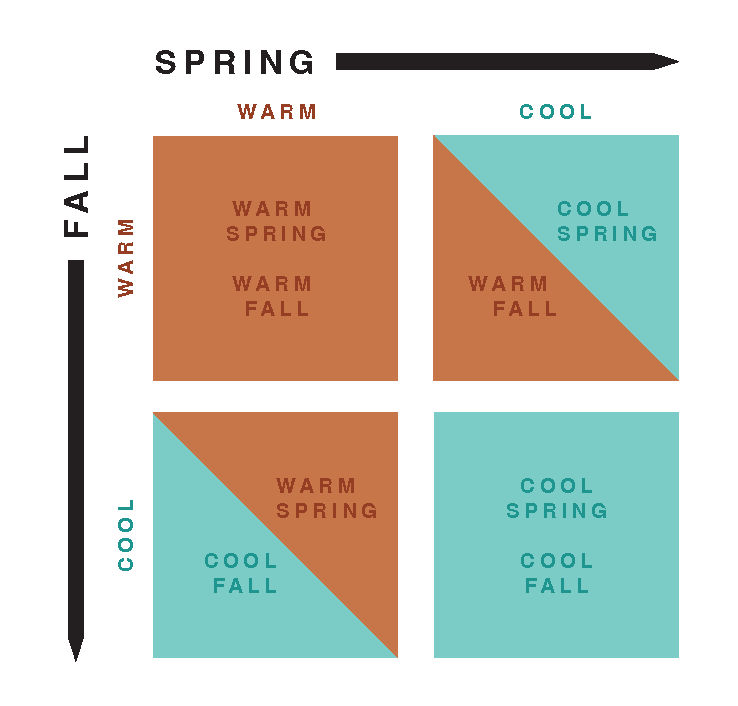
\includegraphics[width=1.1\textwidth]{FullFactorialFigure.pdf} 
\caption{Full factorial design of Cool/Warm Spring and Cool/Warm Fall}
\label{fig:sample}
\end{figure}
%%%
	\item 2-year experiment over 2024-2025 (Fig. 2 and 3)
%%%
\begin{figure}[p]
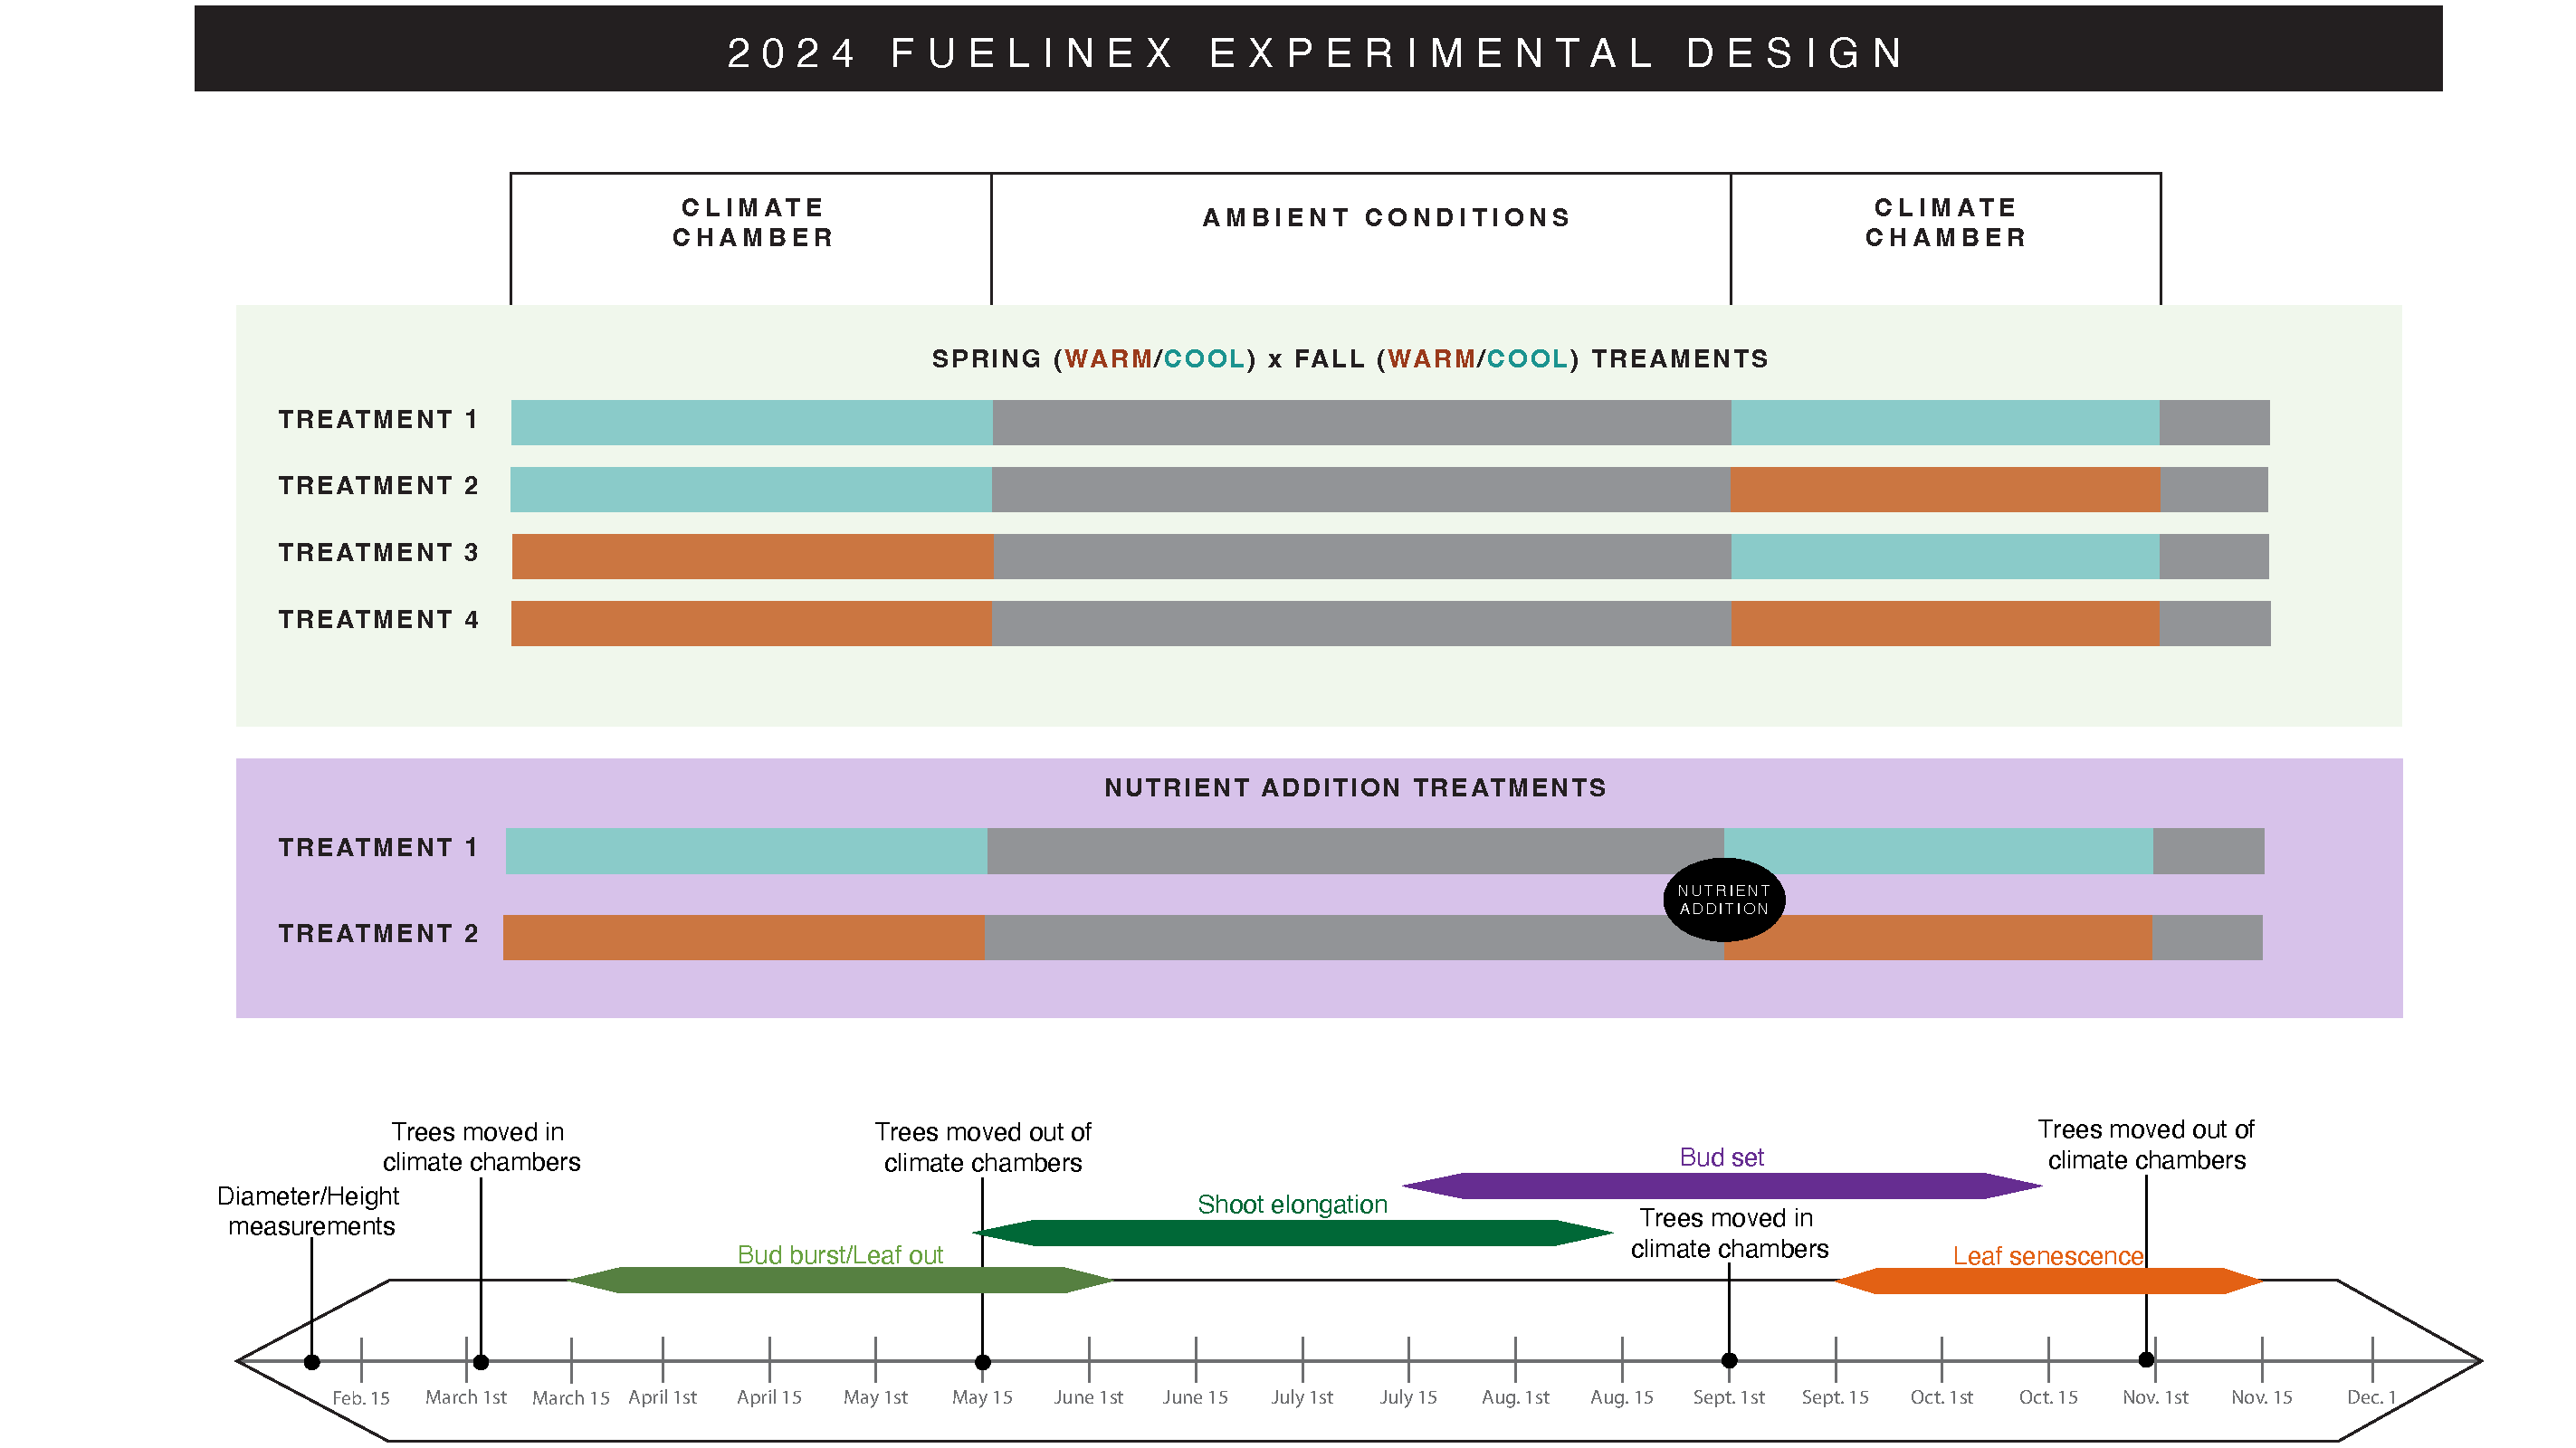
\includegraphics[width=1.1\textwidth]{Fuelinex_Design2024.pdf}
\caption{Experimental design of the different treatments that were performed during the growing season of 2024. The timeline displays the periods of the different measurements. Nutrient addition treatments are displayed by the black elipses}
\label{fig:sample}
\end{figure}
%%%
\begin{figure}[p]
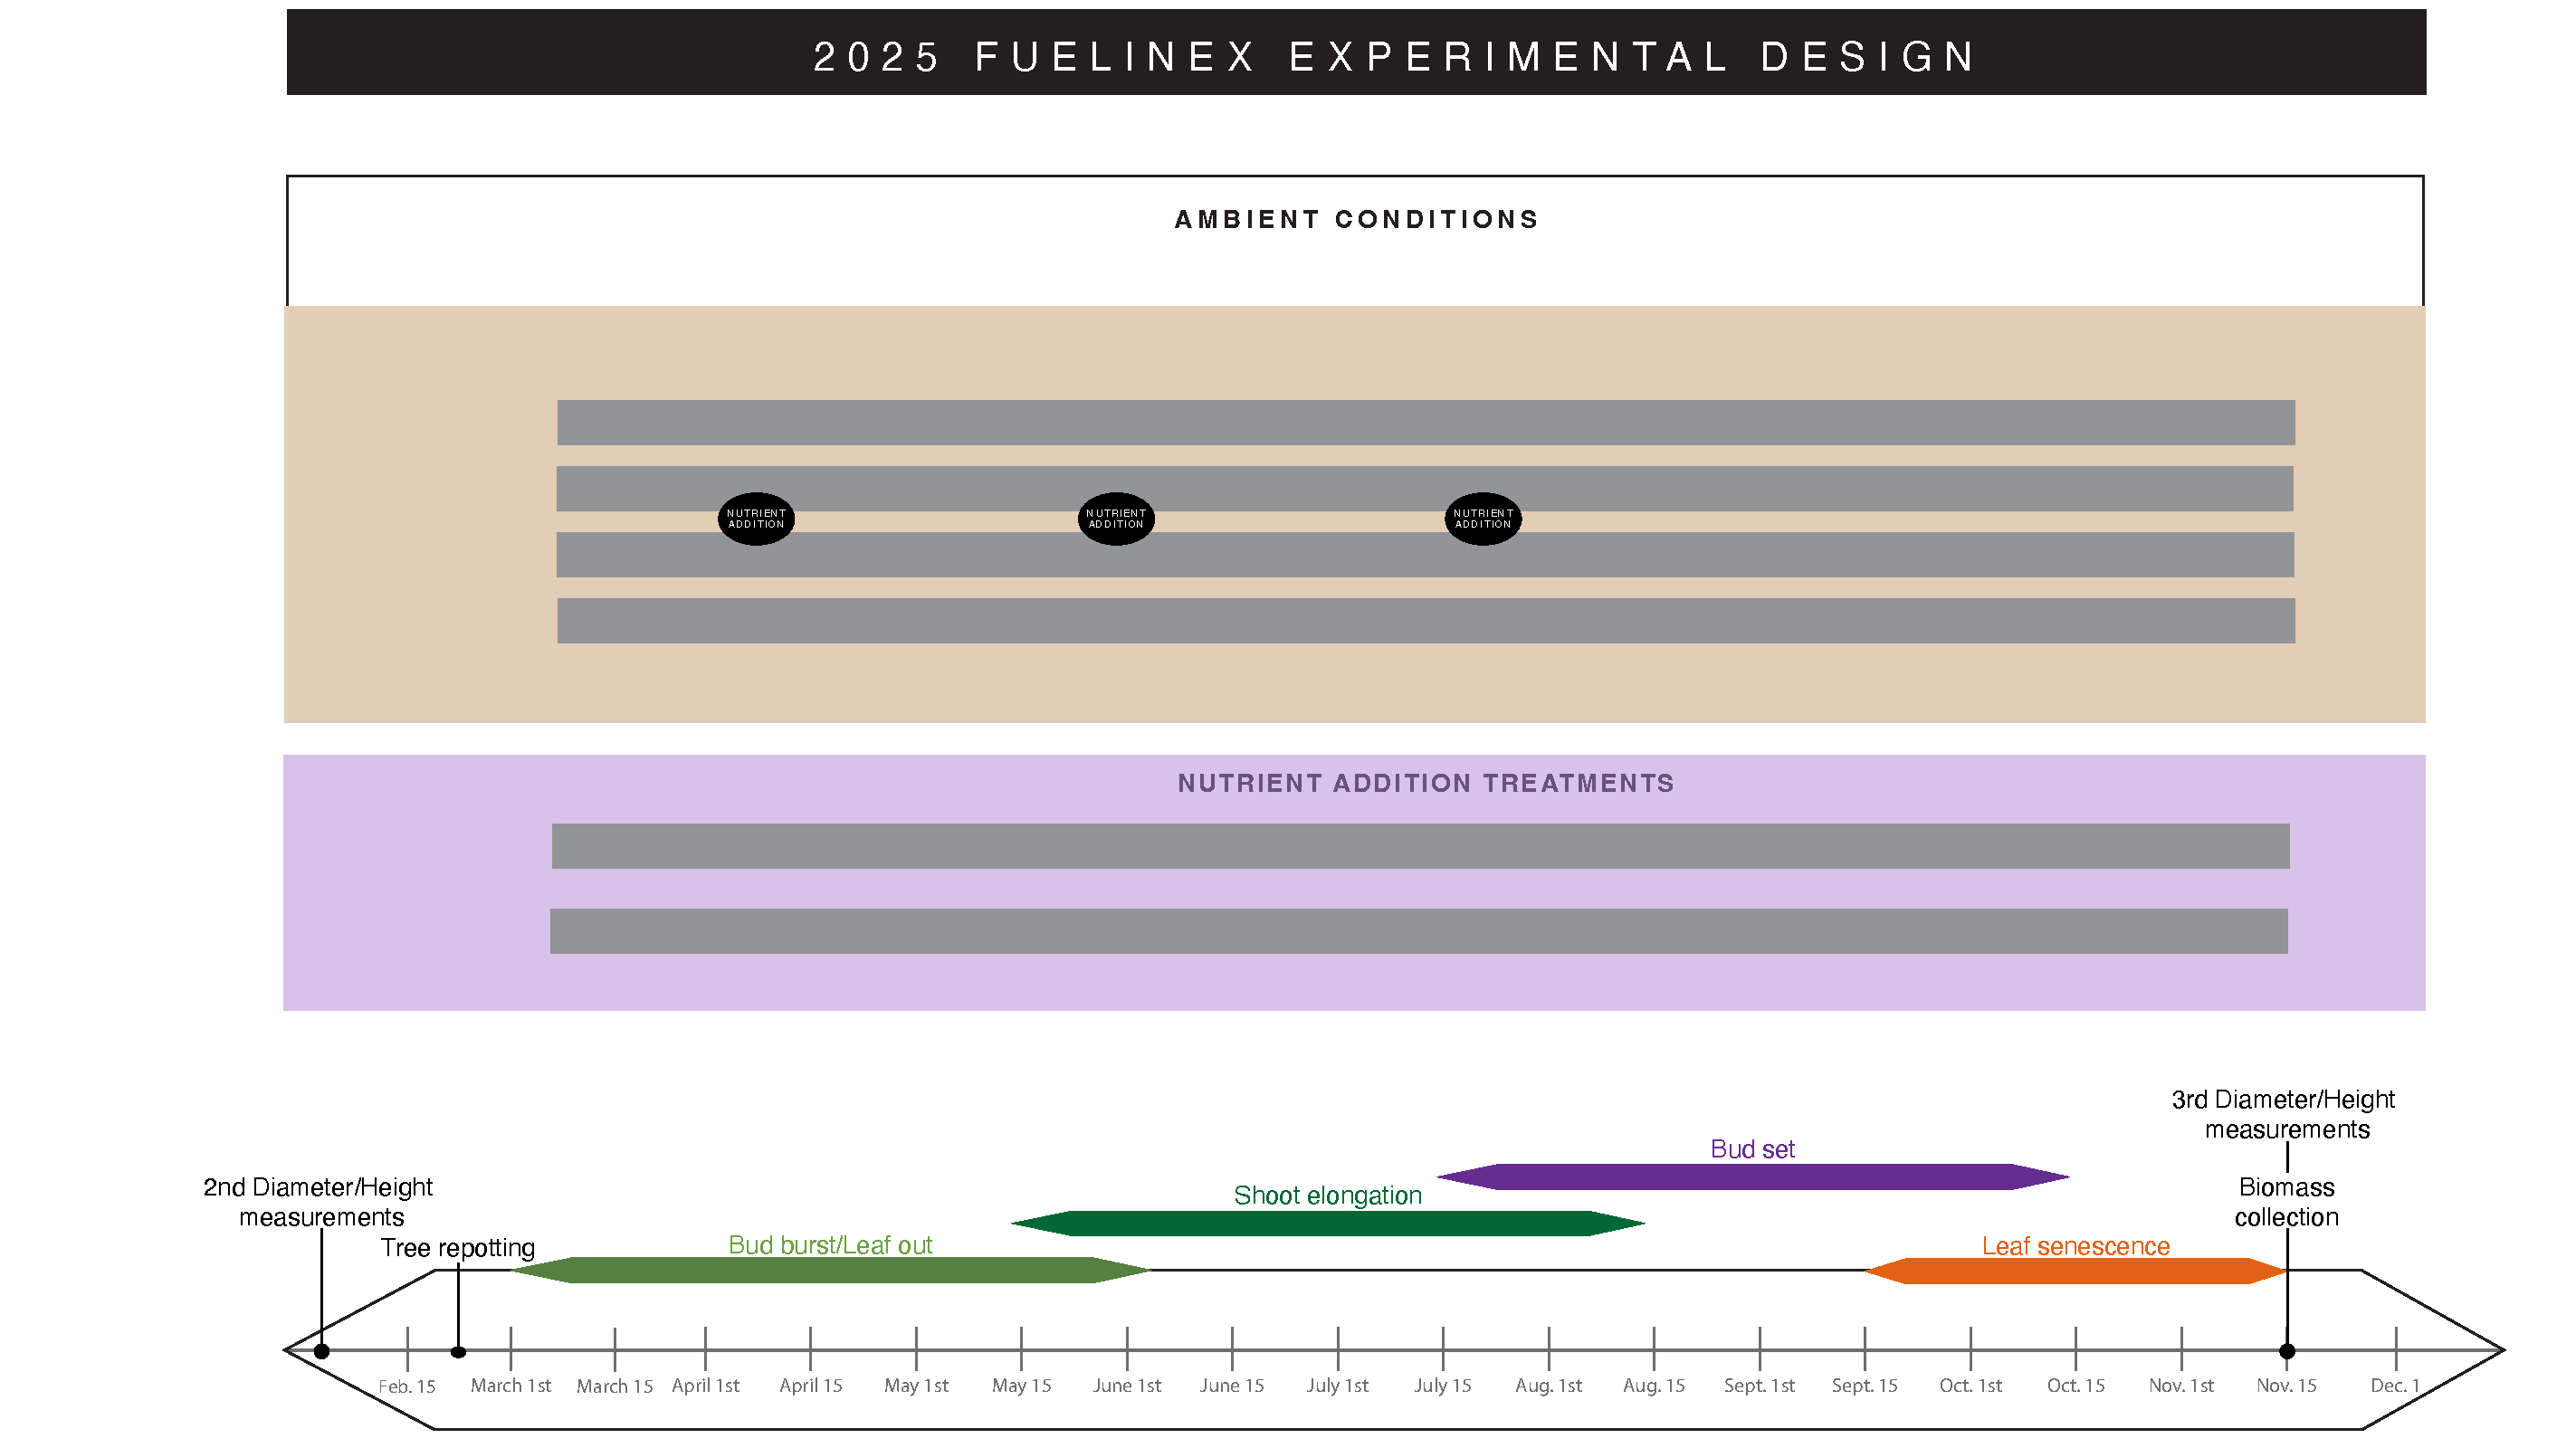
\includegraphics[width=1.1\textwidth]{Fuelinex_Design2025.pdf}
\caption{Timeline displaying the periods of the different measurements during the growing season of 2025}
\label{fig:sample}
\end{figure}
%%%
	\item Nutrient addition
	\item Data: phenology, shoot elongation, diameter, height, biomass, tree rings
	\item Analysis: TBD
	\item Studied species (Table 1)

\end {enumerate}

%%%
\begin{table}[p]
\centering
\caption{Fuelinex species grouped by tree type, life history, and wood anatomy.}
\begin{tabular}{|>{\raggedright\arraybackslash}p{7cm}|p{5cm}|p{3cm}|p{1cm}|}
\hline
\multicolumn{4}{|c|}{\textbf{Deciduous Trees}} \\
\hline
\textbf{Common Name (Latin)} & \textbf{Life History Strategy} & \textbf{Wood Anatomy} & \textbf{n (approx)} \\
\hline
Bur oak (\textit{Quercus macrocarpa}) & Slow-growth, long life & Ring-porous & 87\\
Bitter cherry (\textit{Prunus virginiana}) & Fast-growth, short life & Diffuse-porous & 78\\
Box elder (\textit{Acer negundo}) & Fast-growth, short life  & Diffuse-porous & 90\\
Balsam poplar (\textit{Populus balsamifera}) & Fast-growth, short life  & Diffuse-porous &84 \\
Paper birch (\textit{Betula papyrifera}) & Fast-growth, short life  & Diffuse-porous &90\\
\hline
\multicolumn{4}{|c|}{\textbf{Evergreen Trees}} \\
\hline
White pine (\textit{Pinus strobus}) & Slow-growth, long life & & 89\\
Giant Sequoia (\textit{Sequoiadendron giganteum}) & Slow-growth, long life & & 54\\
\hline
\end{tabular}
\end{table}
%%%
% ============================
% Wildchrokie
% ============================
\subsection{Wildchrokie}
\begin {enumerate}
	\item Common garden from 2015 to 2023
	\item Four species within the Betulacea family (Table 2)
%%%
\begin{table}[p]
\centering
\caption{Wilchrokie species grouped by tree type, life history, and wood anatomy.}
\begin{tabular}{|>{\raggedright\arraybackslash}p{7cm}|p{5cm}|p{3cm}|p{1cm}|}
\hline
\multicolumn{4}{|c|}{\textbf{Deciduous Trees}} \\
\hline
\textbf{Common Name (Latin)} & \textbf{Life History Strategy} & \textbf{Wood Anatomy} & \textbf{n} \\
\hline
Paper birch (\textit{Betula papyrifera}) & Fast-growth, short life  & Diffuse-porous & 8\\
Yellow birch (\textit{Betula alleghaniensis}) & Moderate-growth, moderate life & Diffuse-porous & 21\\
Grey birch (\textit{Betula populifolia}) & Fast-growth, short life & Diffuse-porous & 29\\
Grey alder (\textit{Alnus incana}) & Fast-growth, short life & Diffuse-porous & 31\\
\hline
\end{tabular}
\end{table}
%%%
	\item Data: phenology, height, tree rings
	\item Analysis: Hierarchical model to understand how tree ring width relates to GDD
\end {enumerate}

% ============================
% Treespotters
% ============================
\subsection{Treespotters}
\begin {enumerate}
	\item Citizen science project from 2015 to today (Table 3)
\begin{table}[h]
\centering
\caption{Treespotters species grouped by tree type, life history, and wood anatomy.}
\begin{tabular}{|>{\raggedright\arraybackslash}p{7cm}|p{5cm}|p{3cm}|p{1cm}|}
\hline
\multicolumn{4}{|c|}{\textbf{Deciduous Trees}} \\
\hline
\textbf{Common Name (Latin)} & \textbf{Life History Strategy} & \textbf{Wood Anatomy} & \textbf{n} \\
\hline
American basswood (\textit{Tilia americana}) & Fast-growth, moderate life & Diffuse-porous & 5\\
Eastern cottonwood (\textit{Populus deltoides}) & Fast-growth, short life & Diffuse-porous & 4\\
Northern red oak (\textit{Quercus rubra}) & Moderate-growth, long life & Ring-porous & 4\\
White oak (\textit{Quercus alba}) & Slow-growth, long life & Ring-porous & 5\\
Pignut hickory (\textit{Carya glabra}) & Slow-growth, long life & Ring-porous & 4\\
Shagbark hickory (\textit{Carya ovata}) & Slow-growth, long life & Ring-porous & 4\\
River birch (\textit{Betula nigra}) & Fast-growth, short life & Diffuse-porous & 5\\
Yellow birch (\textit{Betula alleghaniensis}) & Moderate-growth, moderate life & Diffuse-porous & 4\\
Sugar maple (\textit{Acer saccharum}) & Slow-growth, long life & Diffuse-porous & 5\\
Red maple (\textit{Acer rubrum}) & Slow-growth, long life & Diffuse-porous & 4\\
Yellow buckeye (\textit{Aesculus flava}) & Moderate-growth, moderate life & Diffuse-porous & 5\\
\hline
\end{tabular}
\end{table}

	\item Tree coring
	\item Data: phenology, tree rings
	\item Analysis: Hierarchical model to understand how tree ring width relates to GDD	
\end {enumerate}

\section{Timeline} 
Fig. **
%%%
\begin{figure}[h]
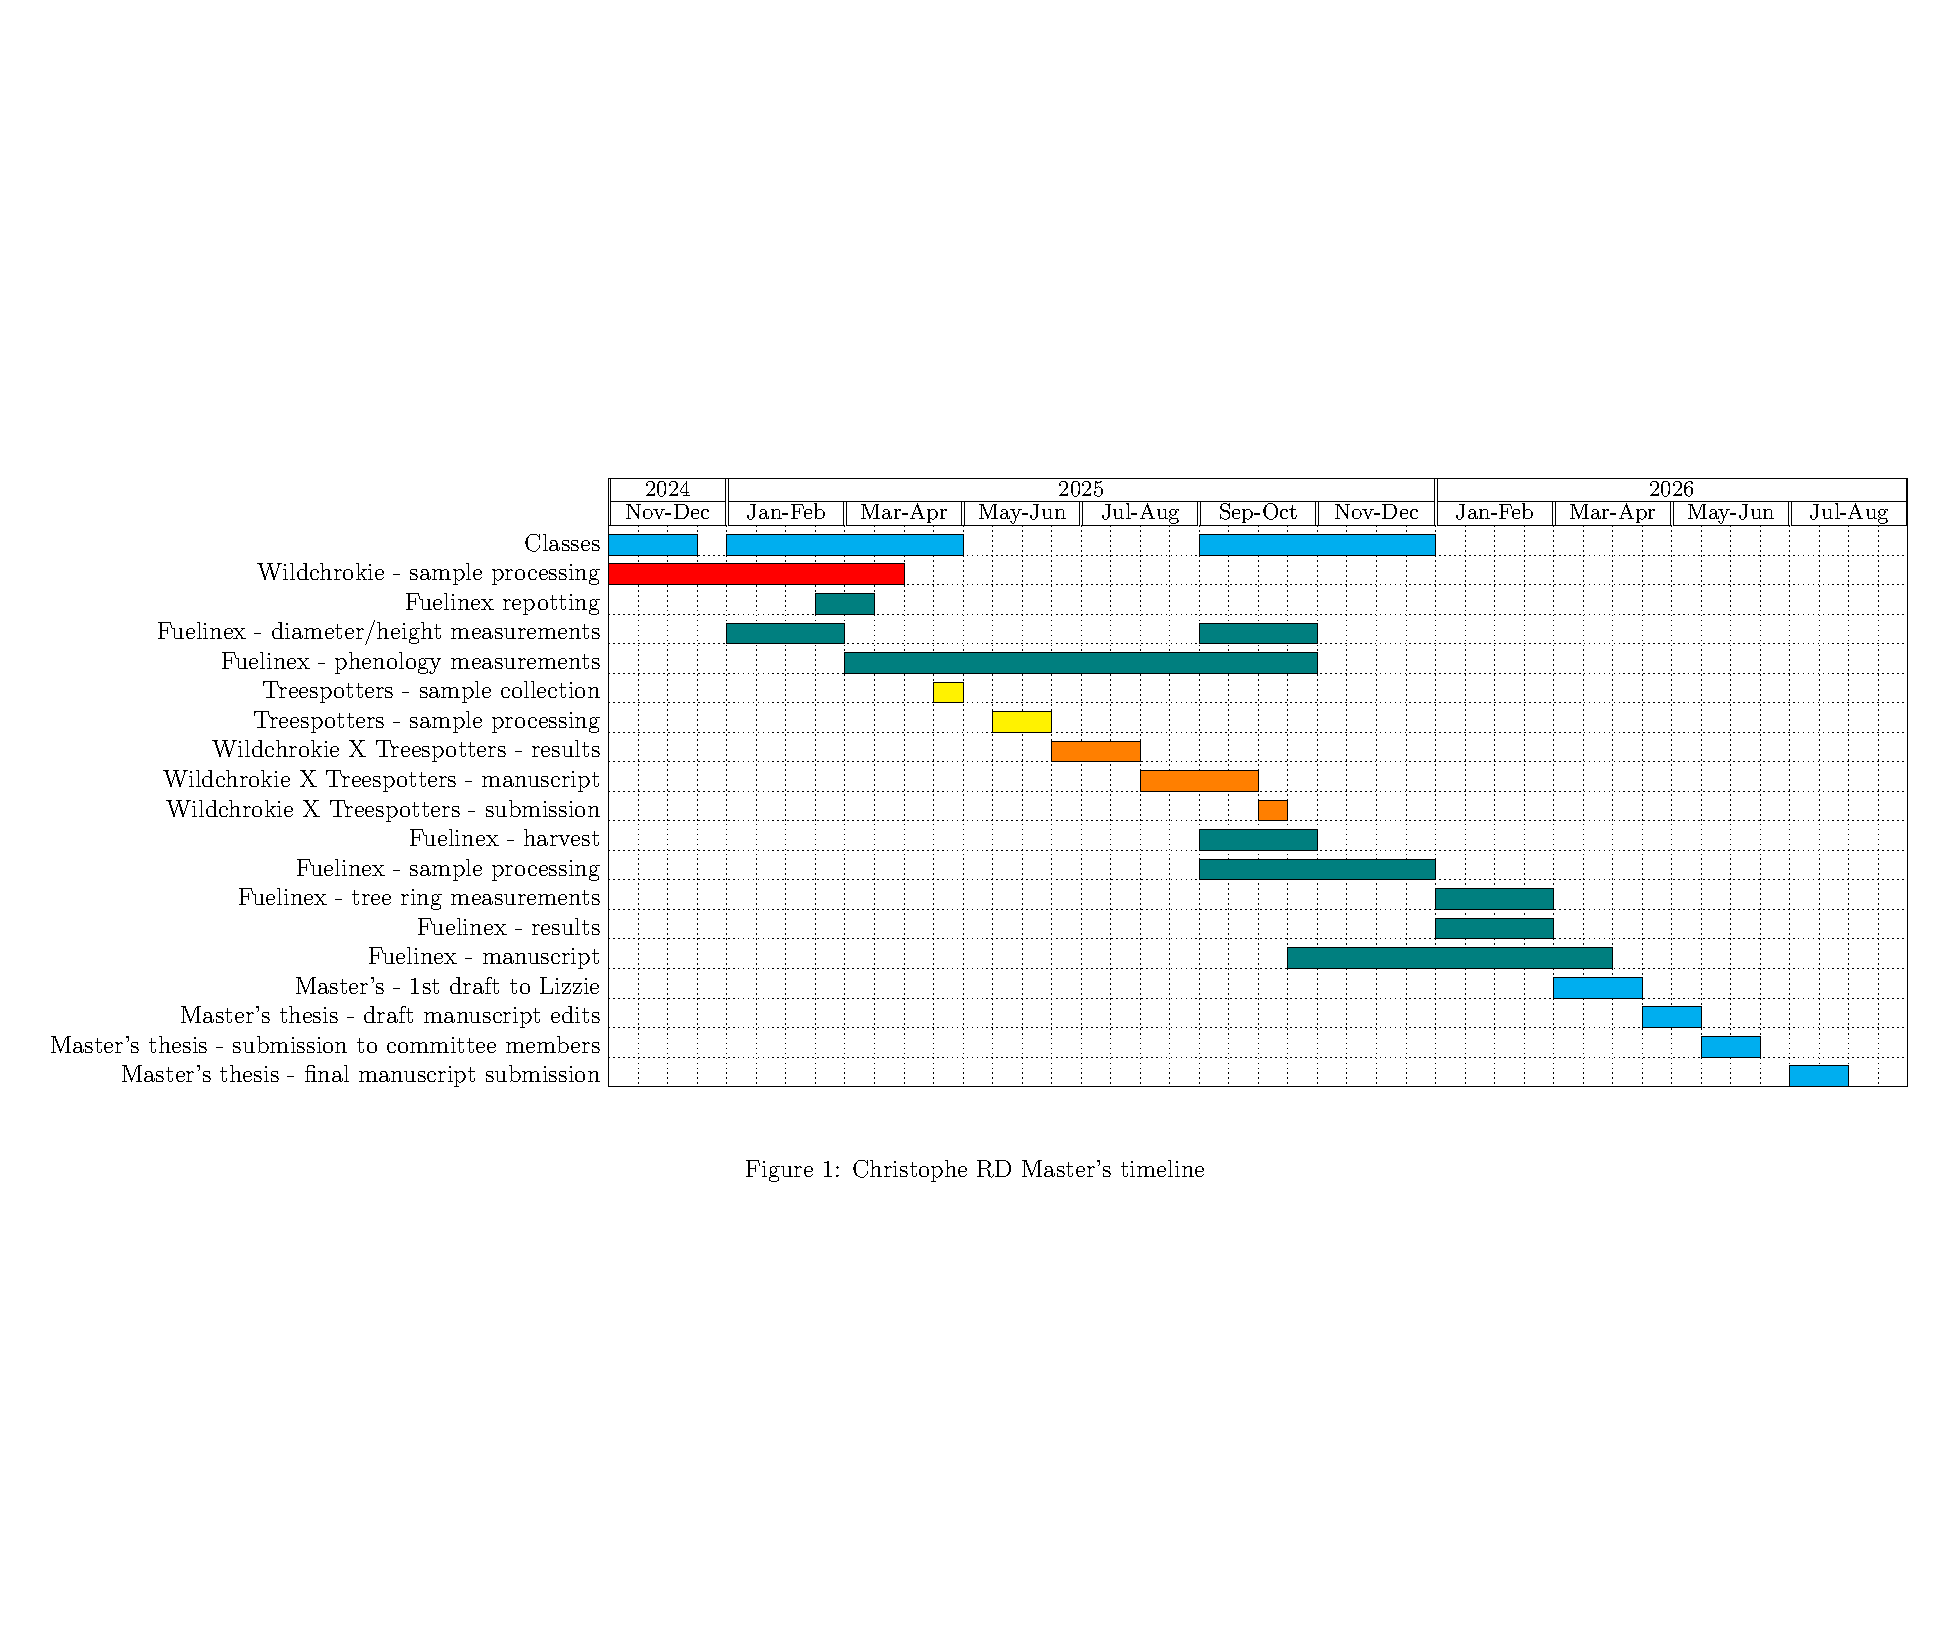
\includegraphics[width=1.1\textwidth]{ganttChart.pdf}
\caption{Gant chart displaying the different milestones to be done over 2025 and 2026}
\label{fig:sample}
\end{figure}
%%%

\section {References}
\bibliography{Exported_Items.bib}
\bibliographystyle{nature} % set citation style 


% old text
%\section*{Chapter 2.1. Wildchrokie: Phenological observations coupling with tree-ring width measurements for a 6-year common garden experiment} While the assumption that a longer growing season leads to increased growth is an intuitive and common one, recent evidence shows that this may not be the case. 
%How phenological season length relates to growth. This is a major question in fundamental biology, but also critical to forecasts of climate change itself, since most carbon models assume that plants experiencing longer seasons will sequester more carbon, but recent studies have called this assumption into question.

\end{document}
